\documentclass[uplatex,dvipdfmx]{jlreq}
\usepackage{threeparttable}
\usepackage[fleqn,tbtags]{mathtools}
\usepackage{jlreq-deluxe}
\usepackage[noalphabet]{pxchfon} % must be after otf package
\usepackage{stix2} %欧文＆数式フォント
%\usepackage{hira-stix} % ヒラギノフォント＆STIX2 フォント代替定義（Warning回避）
\usepackage{url}
\usepackage[hidelinks,dvipdfmx]{hyperref}
\usepackage{here}  % プリアンブルに追加
\usepackage{float}
\usepackage{longtable}
\usepackage{graphicx}
\usepackage{multirow}

\begin{document}

\title{マジカル★観覧車の詳細設計：通信関連の構成}
\author{25G1041 菊池侑人}
%\date{2015年11月13日}
\maketitle

\tableofcontents

\newpage
\section{全体の仕様}
本設計に使用する定数は表\ref{tab:teisuu}の通りである．これらは実装において，プログラム内で const を使って定義する．

\begin{table}[H]
\centering
\caption{設計に利用する定数一覧．}
\label{tab:teisuu}
\begin{tabular}{lllll}
\hline
型 & 名前 & 説明 & 所属 & メモリ量 [byte] \\
\hline
float & VCC & Arduinoへの供給電圧$V_{cc}$ & Main & 4 \\
uint16\_t & LOCAL\_PORT & 通信に利用するポート番号 & SyncManager & 2 \\
char[] & SSID & Wi-Fiのネットワーク名 & SyncManager & Max:33 \\
char[] & PASS & そのWi-Fiのパスワード & SyncManager & Max:64 \\
uint8\_t & PIN\_MOTOR\_PWM & モーター制御用の出力ピン & MotorControl & 1 \\
uint8\_t & bpmTable[] & 5つの離散値BPM格納 & MotorControl & 5 \\
\hline
\end{tabular}
\end{table}

SSIDおよびPASSのメモリ量について，参考文献\cite{ref:Arduino_wifi}によると，Arduino WiFiライブラリではSSIDの最大長を32文字，Wi-Fiパスワード(WPAキー)の最大長を63文字として定義されている．また，Arduino言語を含むC言語やC++の仕様として，文字列の終点を表すヌル文字（\texttt{\textbackslash 0}）を格納するため1バイト分を加算する必要がある．そのため，本設計ではSSIDを33 byte，PASSを64 byteと算出した．

さらに，bpmTable[]の中身は表\ref{tab:bpmtable}のように定義されている．
\begin{table}[H]
\centering
\caption{bpmTable[] に格納するBPM値．}
\label{tab:bpmtable}
\begin{tabular}{c|ccccc}
\hline
インデックス番号 & 0 & 1 & 2 & 3 & 4 \\
\hline
BPM値 & 60 & 90 & 120 & 150 & 180 \\
\hline
\end{tabular}
\end{table}

\paragraph{変数の仕様}
本設計に使用する変数は表\ref{tab:hensuu1}の通りである．

\begin{table}[H]
\centering
\caption{設計に利用する変数一覧．}
\label{tab:hensuu1}
\begin{tabular}{lllll}
\hline
型 & 名前 & 説明 & 所属 & メモリ量 [byte] \\
\hline
uint8\_t & currentBPM & 現在演奏中のBPMデータ & MotorControl & 1 \\
float & RPM & BPMから計算された目標回転数 & MotorControl & 4 \\
float & omega & 目標角速度 $\omega$ & MotorControl & 4 \\
uint8\_t & pwmValue & analogWrite用の出力値 & MotorControl & 1 \\
float & V\_average & 平均電圧$V_{average}$ & MotorControl & 4 \\
\hline
\end{tabular}
\end{table}

\paragraph{関数の仕様}
本設計において，演奏制御および同期処理を実現するために実装する関数を表\ref{tab:function}に示す．

\begin{table}[H]
\centering
\caption{実装する関数の一覧表．}
\label{tab:function}
\begin{tabular}{lllp{6cm}l}
\hline
戻り値 & 関数名 & 引数 & 概要 & 所属 \\ \hline
void & receiveUDP & なし & 指揮デバイスから送信されるBPMの段階番号を受信する．受信されたデータは currentBPM に格納する & SyncManager \\ \hline
void & startRamp & なし & 演奏開始時の加速を制御する．予約されたBPMに基づき1小節分の時間をかけて徐々に目標速度（RPM）へ到達させる． & MotorControl \\ \hline
void & changeBPM & uint8\_t & 演奏中のBPM変更を行う． & MotorControl \\ \hline
\end{tabular}
\end{table}

今後の説明では，表\ref{tab:function}で定義した関数を用いて処理ロジックを述べる．

\paragraph{Arduinoのメモリの検証}
本設計がターゲットハードウェアのメモリ制約を満たすか検証を行う．使用するマイコンボードはArduino UNO R4 WiFi である．データシートによれば，本機に搭
載されているマイコンは，プログラムの実行中に変数や計算結果を保持するSRAM を32 KB，プログラム本体を保存するFlash メモリを256 KB 備えている\cite{ref:Arduino_memori}．

表\ref{tab:teisuu}表および\ref{tab:hensuu1}に示した通り，本システムのメモリ使用量は 123 byte である．
これはSRAM 全体の約0.3\% 程度に留まっており，無線通信ライブラリや制御スタックによる動的なメモリ消費を考慮しても，十分な容量を確保できていると判断した．

\section{通信機能の設計}
\subsection{全体の概要}
本設計では，Wifiを用いたUDPによる通信と，物理同期LEDを用いた同期を行っている．通信の概要を図\ref{fig:gaiyou}に示す．
\begin{figure}[H]
  \centering
  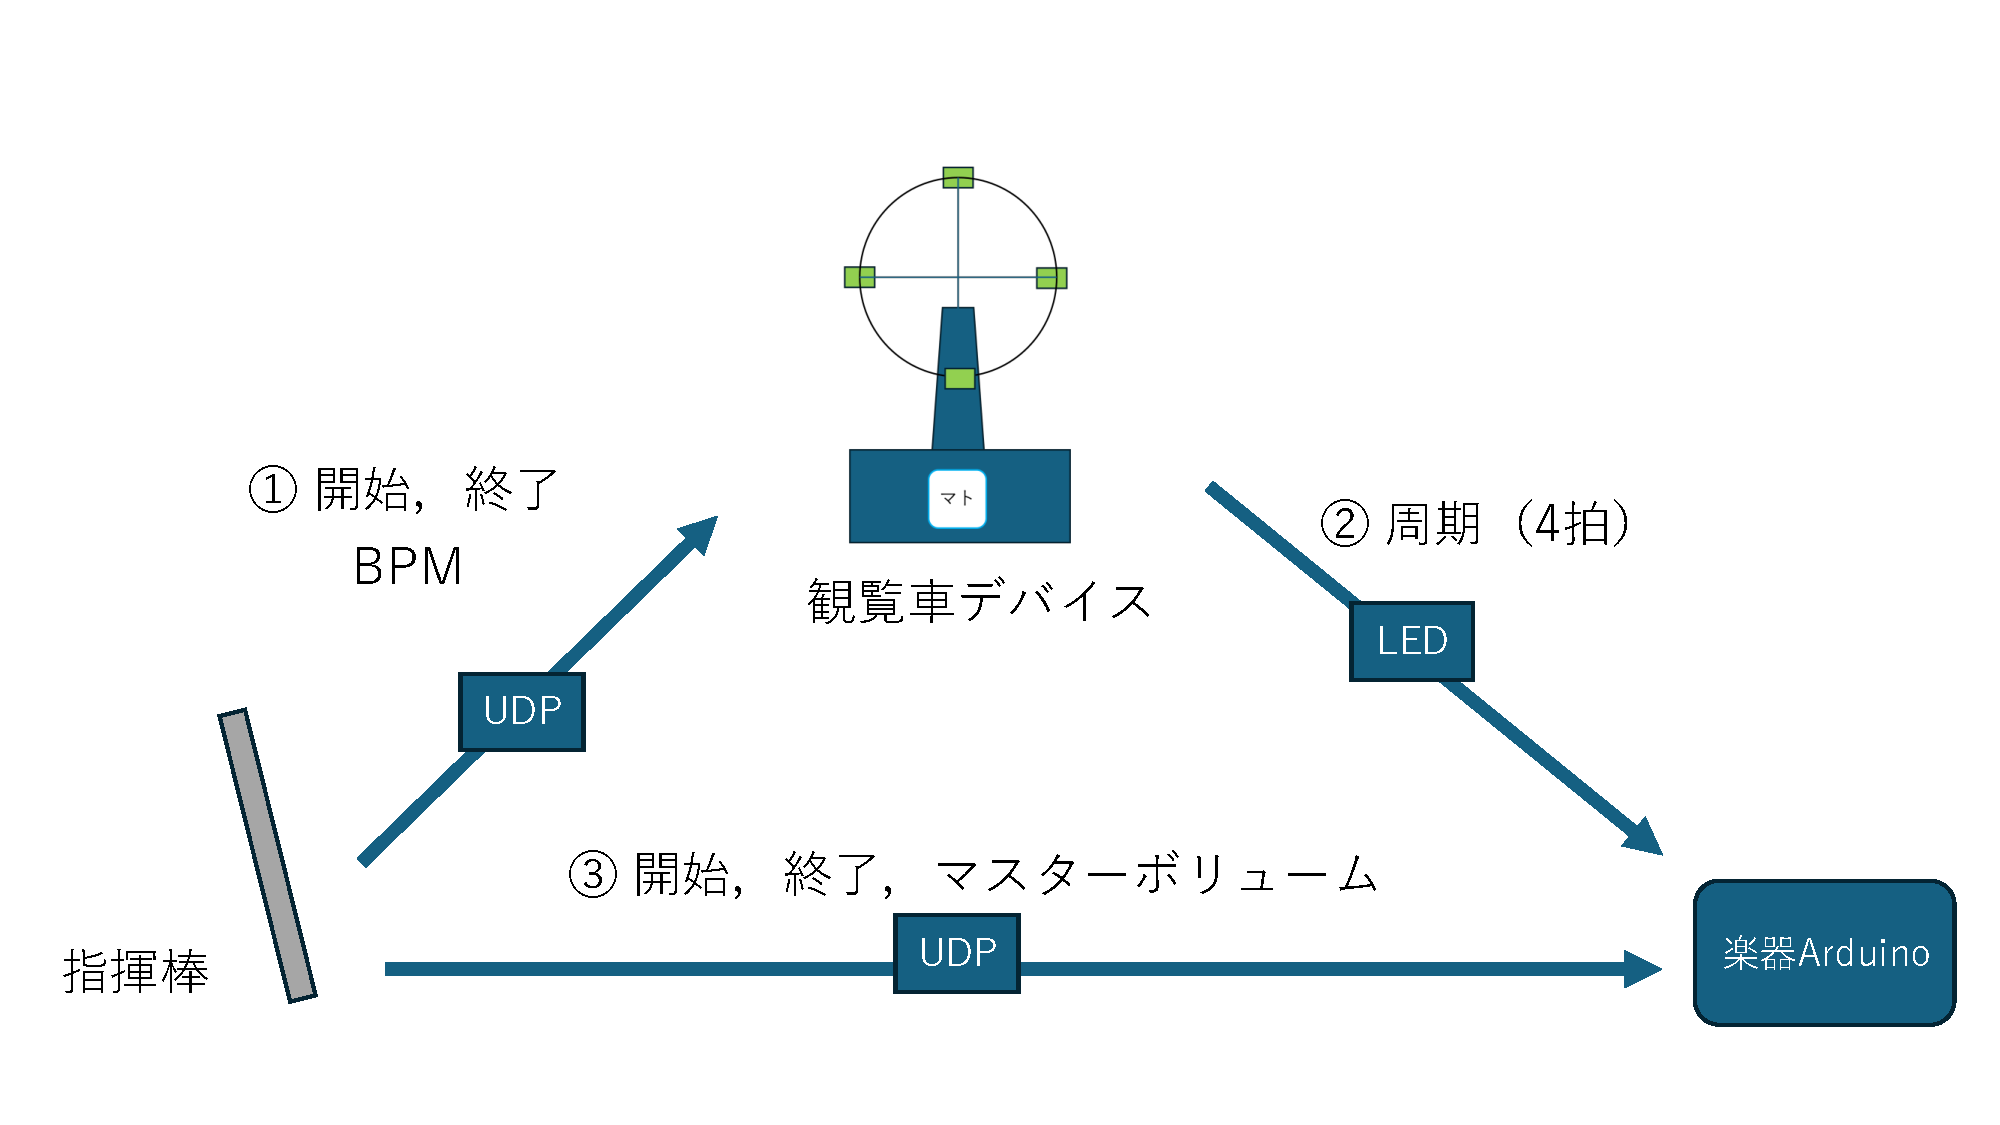
\includegraphics[width=0.8\linewidth]{gaiyou.pdf}
  \caption{本システムの通信経路の概要．}
  \label{fig:gaiyou}
\end{figure}

\subsection{無線通信仕様(UDP)}
無線通信は，利用するマイコンであるArduino UNO R4 WiFiに合わせるためWiFiS3.hライブラリを使用する．
指揮デバイス(指揮棒)を送信元とし，中継機へはBPMの段階番号を，楽器へはタイミングをずらしながら開始信号(ヘッダ)と音量をユニキャストで個別に送信する仕様とする．なお，終了時の演奏終了ヘッダは両方に送信する．
指揮デバイスに搭載された可変抵抗器（BPM，音量をユーザーが操作する用）および指揮棒(加速度センサを搭載した開始・終了検知用）の状態に基づき，表\ref{tab:range}のように電圧値から変換された1～5の段階番号や制御コマンドを受信する．

\begin{table}[H]
\centering
\caption{段階と入力値範囲の対応表．}
\label{tab:range}
\begin{tabular}{c|c}
\hline
段階 & 入力値の範囲 \\ \hline
1 & 0 -- 204 \\ \hline
2 & 205 -- 409 \\ \hline
3 & 410 -- 614 \\ \hline
4 & 615 -- 819 \\ \hline
5 & 820 -- 1023 \\ \hline
\end{tabular}
\end{table}

受信した段階番号を元に，中継機および楽器デバイスは表\ref{tab:bpm_volume}のような変換をする．
\begin{table}[H]
\centering
\caption{各段階に対応するBPMおよび音量設定値．}
\label{tab:bpm_volume}
\begin{tabular}{c|c|c}
\hline
段階 & BPM 設定値 & 音量設定値 \\ \hline
1 & 60 & 0 \\ \hline
2 & 90 & 64 \\ \hline
3 & 120 & 128 \\ \hline
4 & 150 & 192 \\ \hline
5 & 180 & 255 \\ \hline
\end{tabular}
\end{table}

パケットの構造は表\ref{tab:hed}，表\ref{tab:payload}のように，識別用のヘッダとデータ本体からなる合計2 バイトの固定長ペイロードとして定義する．
\begin{table}[H]
\centering
\caption{通信の識別ヘッダ．(第1バイト:char)}
\label{tab:hed}
\begin{tabular}{c|c|l}
\hline
ヘッダ & 値（ASCIIコード） & 内容 \\ \hline
`'B'` & 0x42 & BPMデータ \\ \hline
`'V'` & 0x56 & 音量データ \\ \hline
`'S'` & 0x53 & 演奏開始（Start） \\ \hline
`'E'` & 0x45 & 演奏終了（End） \\ \hline
\end{tabular}
\end{table}

\begin{table}[H]
\centering
\caption{各ヘッダに対応したペイロードの内容．(第2バイト:uint8\_t)}
\label{tab:payload}
\begin{tabular}{c|l}
\hline
ヘッダ & ペイロード内容 \\ \hline
`'B'` & BPM の段階番号（1～5）を受信．中継機内部の \texttt{bpmTable[]} を参照し，設定値へ変換． \\ \hline
`'V'` & 音量 の段階番号（1～5）を受信．楽器ユニットへ送信される． \\ \hline
`'S'` & 演奏開始コマンド．各楽器ユニットが受信し，このパケットの到達をトリガーとして即座に演奏を開始． \\ \hline
`'E'` & 演奏終了コマンド．第2バイトにはダミーデータ（0）が格納されており，受信後は停止処理へ移行． \\ \hline
\end{tabular}
\end{table}

UDPは到達保証がないプロトコルなので，システムの信頼性を高めるために次のような設計を採用する．
\begin{itemize}
    \item 冗長送信: パケットロスによる制御の失敗を防ぐため，BPM変更，演奏開始・終了の各イベント発生時に，短い間隔(例えば20 ms)で同一パケットを3 回連続して送信する仕様とする．
    \item 送信タイミング: 指揮デバイスの状態（BPM・音量の段階）が変化した瞬間に即時送信を行う．状態に変化がない間はパケット送信を行わないことで，ネットワーク帯域の占有を最小限に抑える．
\end{itemize}
ここで20 msは，BPM120の1拍（500ms）に対して十分短い時間なため，リズムのズレとして許容できる．

\subsection{物理同期信号の設計(LED)}
各カゴに搭載されたLEDは常に点灯される．観覧車の回転に伴って，LEDが楽器側の照度センサーを通過する際の光の立ち上がりを物理的な同期パルスとして利用する．
本設計では1象限の移動を1小節と定義しているため，このパルス検知は各小節の第1拍の開始を意味している．

楽器ユニット側は，演奏開始前の空転時間において，このパルスの検出間隔から事前に実際のBPMを計算して演奏待機状態とする．実際の演奏開始は，指揮デバイスから個別に送信される演奏開始パケット（ヘッダ\texttt{'S'}'）を受信した瞬間をトリガーとする．2回目以降のパルス検知は，物理的な回転速度のズレを補正するための基準信号として利用する設計とする．

\section{ソフトウェア設計}
\subsection{ファイル構成}
各役割ごとに，ファイルを次のように定義する．
\begin{itemize}
    \item FerrisWheel.ino: メインロジックを担当する．\texttt{loop}関数におけるUDP受信処理や変速処理の呼び出しなどを行う．
    \item MotorControl.cpp:モーターの制御を行う．ルックアップテーブルに基づく回転速度の切り替えや，起動時の加速を担当する．
    \item MotorControl.h:MotorControl.cppのヘッダーファイルを定義する．
    \item SyncManager.cpp:通信を行う．指揮デバイスからのUDPパケットの受信処理を行う．
    \item SyncManager.h:SyncManager.cppのヘッダーファイルを定義する．
\end{itemize}

\subsection{オブジェクト設計}
\subsubsection{クラス図}
本設計におけるクラス図を図\ref{fig:class}のように定義する．

\begin{figure}[H]
  \centering
  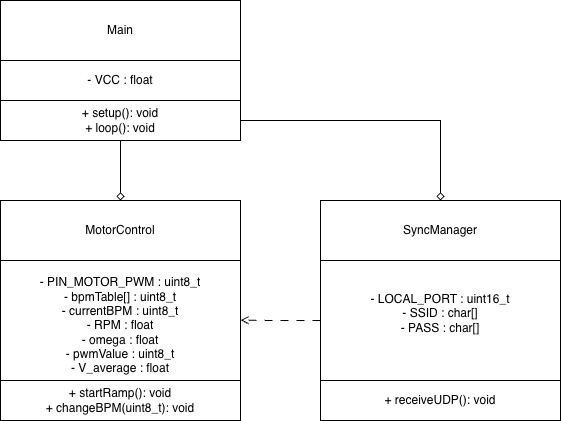
\includegraphics[width=0.8\linewidth]{classzu.png}
  \caption{本システムのクラス図．}
  \label{fig:class}
\end{figure}
メインとなる \texttt{Main} クラスが全体の進行を管理し，モータ制御を担う \texttt{MotorControl} クラスと通信・同期を担う \texttt{SyncManager} クラスを集約（所有）する構成とした．これにより，各機能の独立性を高めつつ，システム全体の司令を明確にしている．

\section{処理フローの設計}
\subsection{LEDを用いた演奏同期機能設計}
ここでは，楽器の目の前をカゴが通過する瞬間に，正確に同期信号を楽器に送ることを目的とする．本機能は，通信クラスである \texttt{SyncManager} によって管理される．
\paragraph{同期のメカニズム}
本設計では，観覧車の電源に直接接続された，土台側に配置された4つのLEDを常に点灯させておく．これに対して，楽器ユニットは固定されているため，観覧車の回転運動によってLEDが照度センサの正面を横切る瞬間のみ，センサ側で受光エネルギーの変化（物理パルス）が観測される．この一連の仕組みを図\ref{fig:LED}に示す．
\begin{figure}[H]
  \centering
  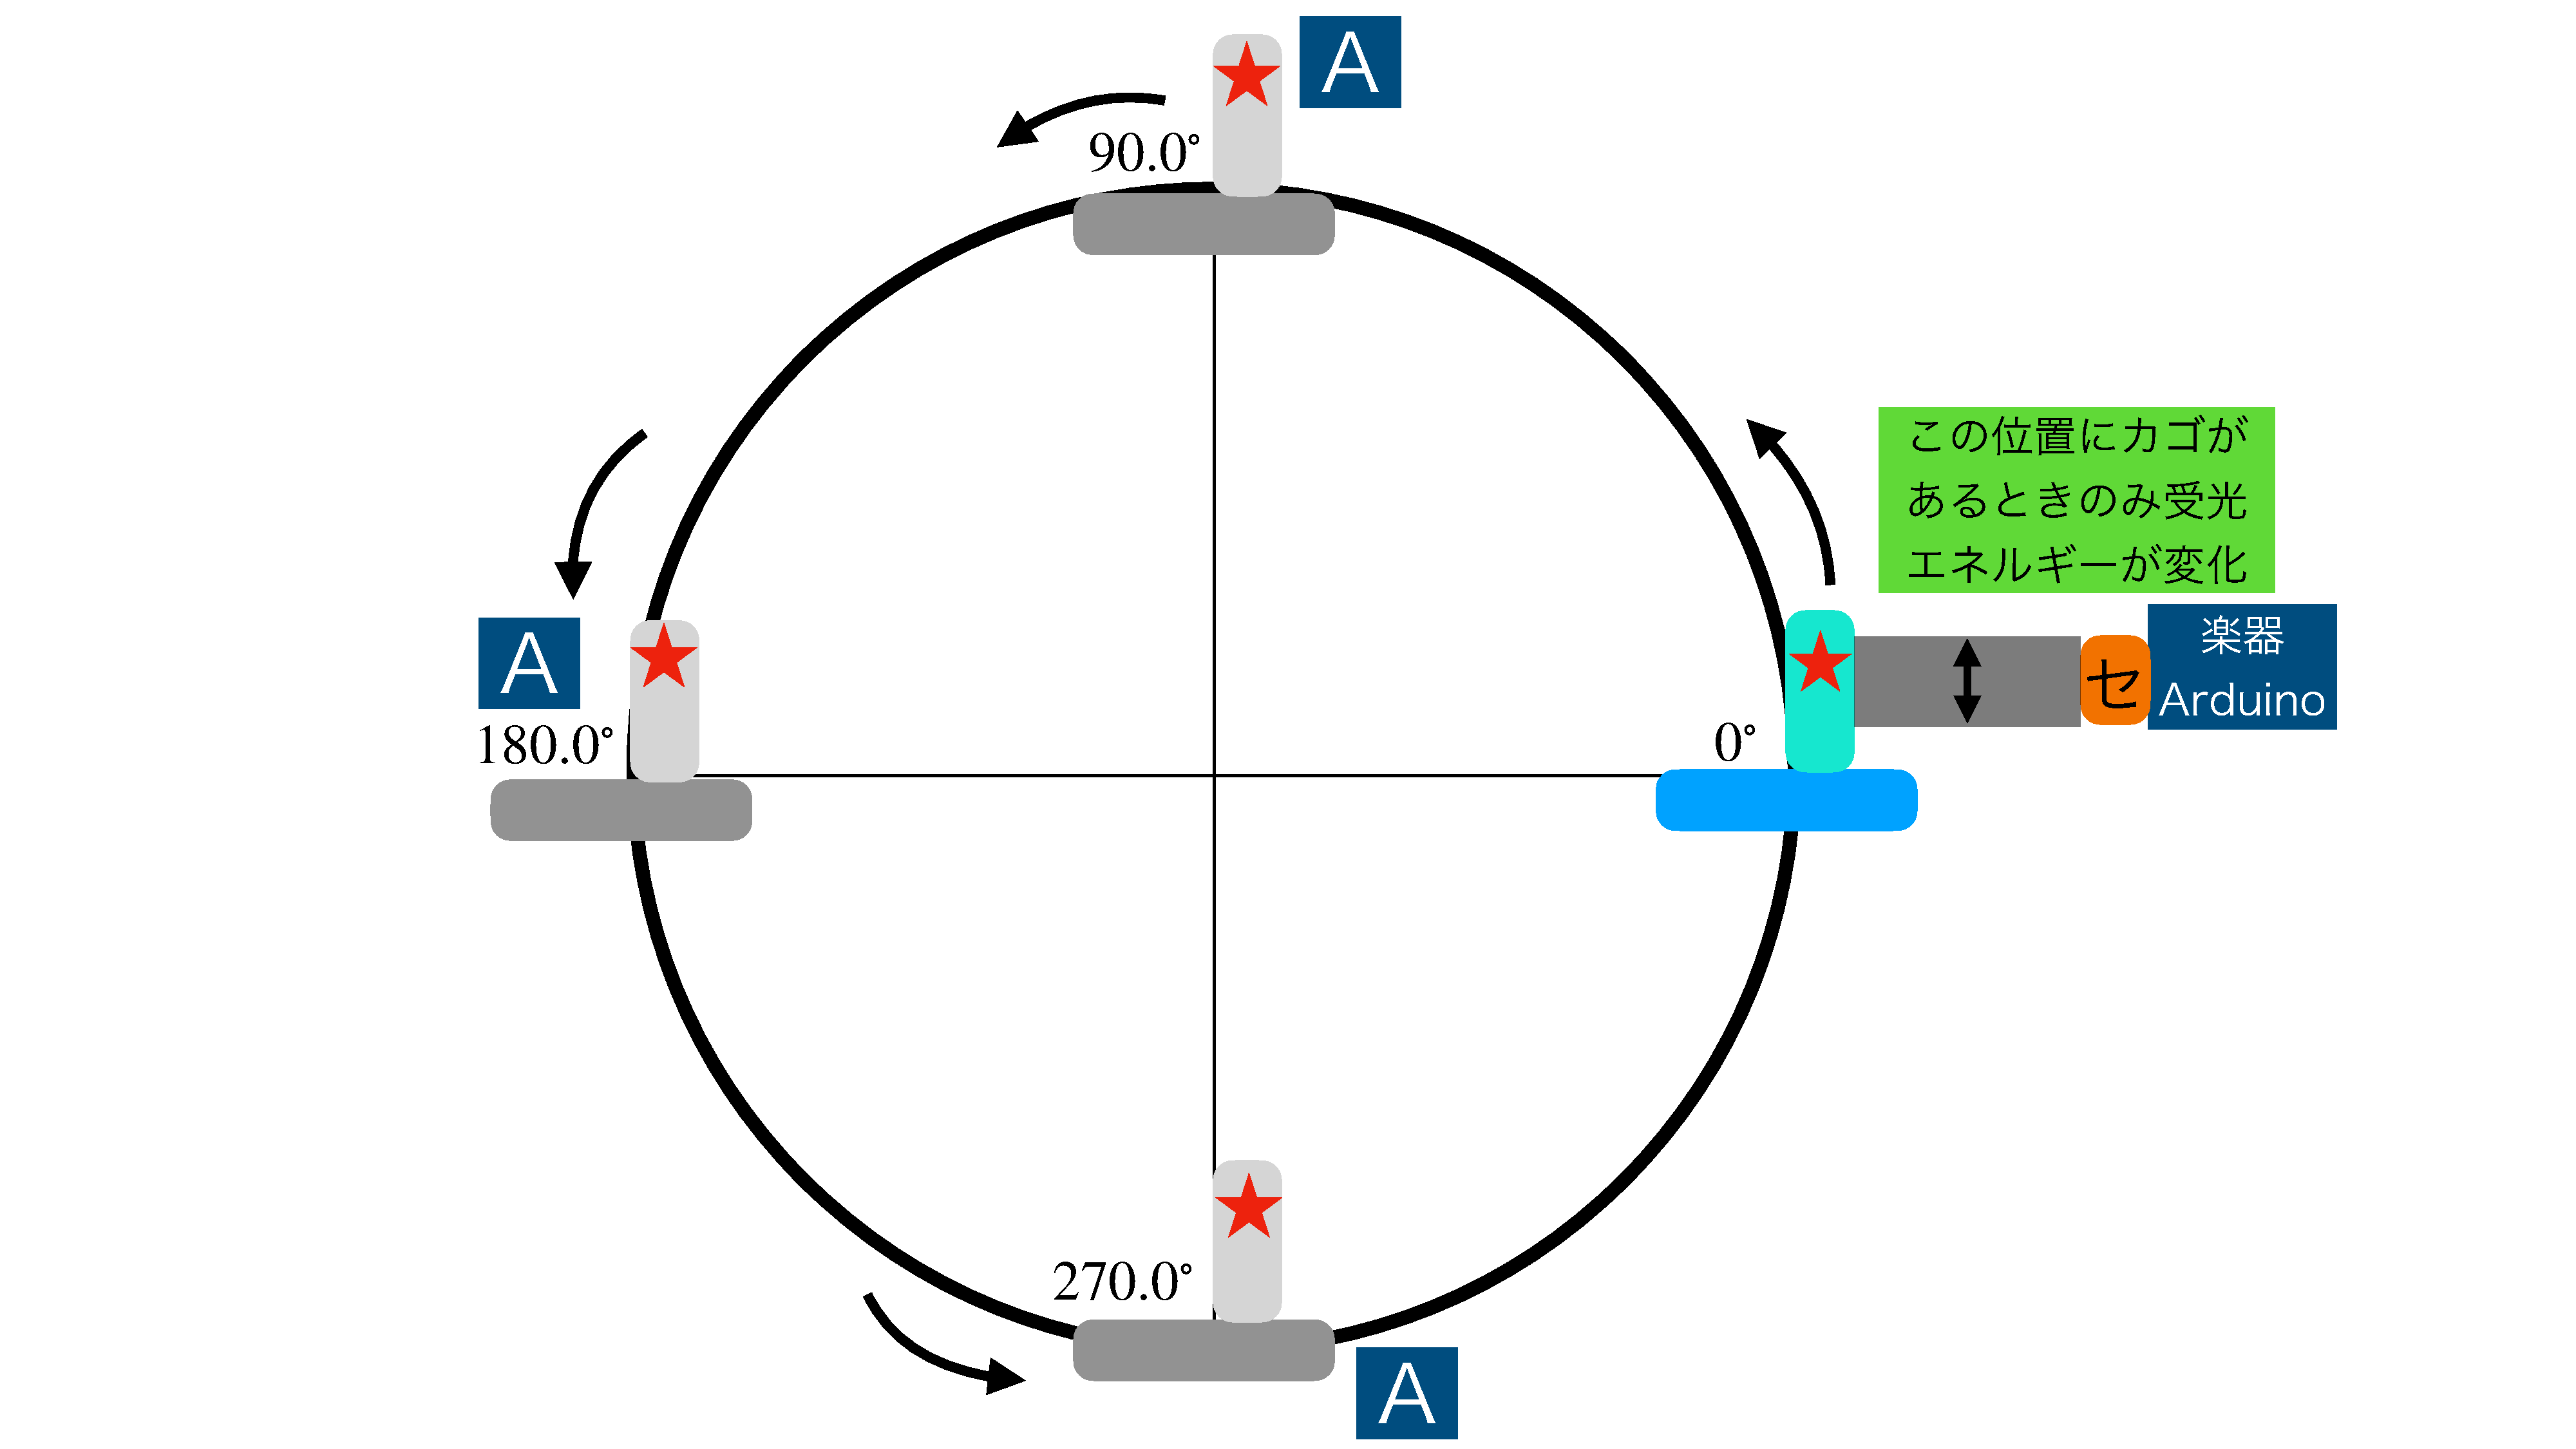
\includegraphics[width=0.8\linewidth]{LED.pdf}
  \caption{同期システムの概念図．}
  \label{fig:LED}
\end{figure}
4拍子の曲において1小節で1象限（$90^\circ$）回転するという条件では，各楽器が1拍目の基準を検知する物理的な角度は表\ref{tab:kakudo}の通りである．
\begin{table}[H]
\centering
\caption{各LED（センサ）の配置角度．}
\label{tab:kakudo}
\begin{tabular}{c|c}
\hline
LED番号 & 配置角度 \\ \hline
LED1 & $0^\circ$ \\
LED2 & $90^\circ$ \\
LED3 & $180^\circ$ \\
LED4 & $270^\circ$ \\ \hline
\end{tabular}
\end{table}
これにより，演算や通信の遅延に影響されず，物理現象に基づく確実な同期を実現する．
楽器ユニット側は，演奏開始前の時間にこのパルスが検出される時間間隔（周期）から現在のBPMを自動で逆算し，演奏待機状態とする．
なお，演奏開始後における2拍目以降のタイミングについては，楽器側でこの物理パルスを基準に内部Tickを補正し，生成する仕様となっている．

\subsection{回転速度同期機構の設計}
\paragraph{モータ制御の原理とBPMの変換}
ここでは，BPMという数字を，実際の回転数\texttt{RPM}に変換させることを目的とする．
本システムでは，ArduinoのPWM（パルス幅変調）機能を用いてモータの平均印加電圧を制御する．供給電圧を $V_{cc}$（定数 \texttt{VCC}），プログラム上の出力値を $pwmValue$ とすると，モータに加わる平均電圧 $V_{average}$ は(\ref{eq:average})式で決定される．
\begin{equation}
\label{eq:average}
V_{average} = V_{cc} \times \frac{pwmValue}{256}
\end{equation}
また，BPMをモータの目標回転数 \texttt{RPM} へ変換するロジックを定義する．本システムでは，4拍で90度回転する仕様に基づき，\texttt{RPM}は(\ref{eq:rpmteigi})式で表せ，1回転の時間は(\ref{eq:ssteigi})式で求められる．
\begin{equation}
\label{eq:rpmteigi}
  RPM = \frac{BPM}{16}
\end{equation}
\begin{equation}
\label{eq:ssteigi}
  60 \div RPM = 60 \div \frac{BPM}{16} = \frac{960}{BPM}
\end{equation}
制御の指標となる角速度\texttt{omega}($\omega$)は(\ref{eq:omegateigi})式で求められる．
\begin{equation}
\label{eq:omegateigi}
\omega = 360^\circ \div \frac{960}{BPM} = \frac{3}{8}BPM
\end{equation}

\paragraph{ルックアップテーブルによる速度制御}
一般的なDCモータの回転速度は供給電圧に比例する性質があるが\cite{ref:control}，実際には摩擦や機構の負荷などによる非線形な挙動を示す事が多い．
そのため近似直線を用いる手法ではなく，より確実な速度追従を実現するため，実測値に基づくルックアップテーブル方式を採用する．

\texttt{MotorControl} クラスは，表\ref{tab:pwm_lut}に示す離散的な5段階のBPM設定値を保持し，受信した段階番号に応じた \texttt{pwmValue} を即座に選択・出力する構成とする．
\begin{table}[H]
\centering
\caption{BPMに対する目標RPMと実測出力PWM値}
\label{tab:pwm_lut}
\begin{tabular}{c|c|c|c}
\hline
段階 & 目標BPM & 目標RPM & 出力PWM値 \\ \hline
1 & 60 & 3.75 &（実測値A）\\
2 & 90 & 5.625 &（実測値B）\\
3 & 120 & 7.5 &（実測値C）\\
4 & 150 & 9.375 &（実測値D）\\
5 & 180 & 11.25 &（実測値E）\\ \hline
\end{tabular}
\end{table}
目標RPMは(\ref{eq:rpmteigi})式から算出している．ここからは実測値の測定方法について説明する．ただし，このロジックはシステムに本実装するプログラムではなく，測定方法であることに注意する．
まず，1象限分回る時間($T_{target}$)を(\ref{eq:target})式で計算する．
\begin{equation}
\label{eq:target}
    T_{target} = \frac{60}{BPM} \times 4
\end{equation}
そこから，任意のPWM 値でモーターを回し，実験用の外部計測器等を用いてカゴが1象限を通過する時間を\texttt{millis()}関数等を用いて測定する．この測定時間が$T_{target}$に限りなく近づくまでPWM 値を微調整する．


\subsection{演奏制御機能設計}
\paragraph{開始時の動作}
ここでは，音楽と回転の同時スタートを管理することを目的とする．具体的には，指揮デバイスからBPMの段階番号を受信したあと，観覧車が目標速度で安定空転する時間を設け，楽器側にBPMを測定させる設計としている．

本ロジックは，観覧車の電源が投入され，かつ指揮デバイスからBPMの段階番号を受信した際に行われる．
まず，受信時の動作を図\ref{fig:jusin}に示す．
\begin{figure}[H]
  \centering
  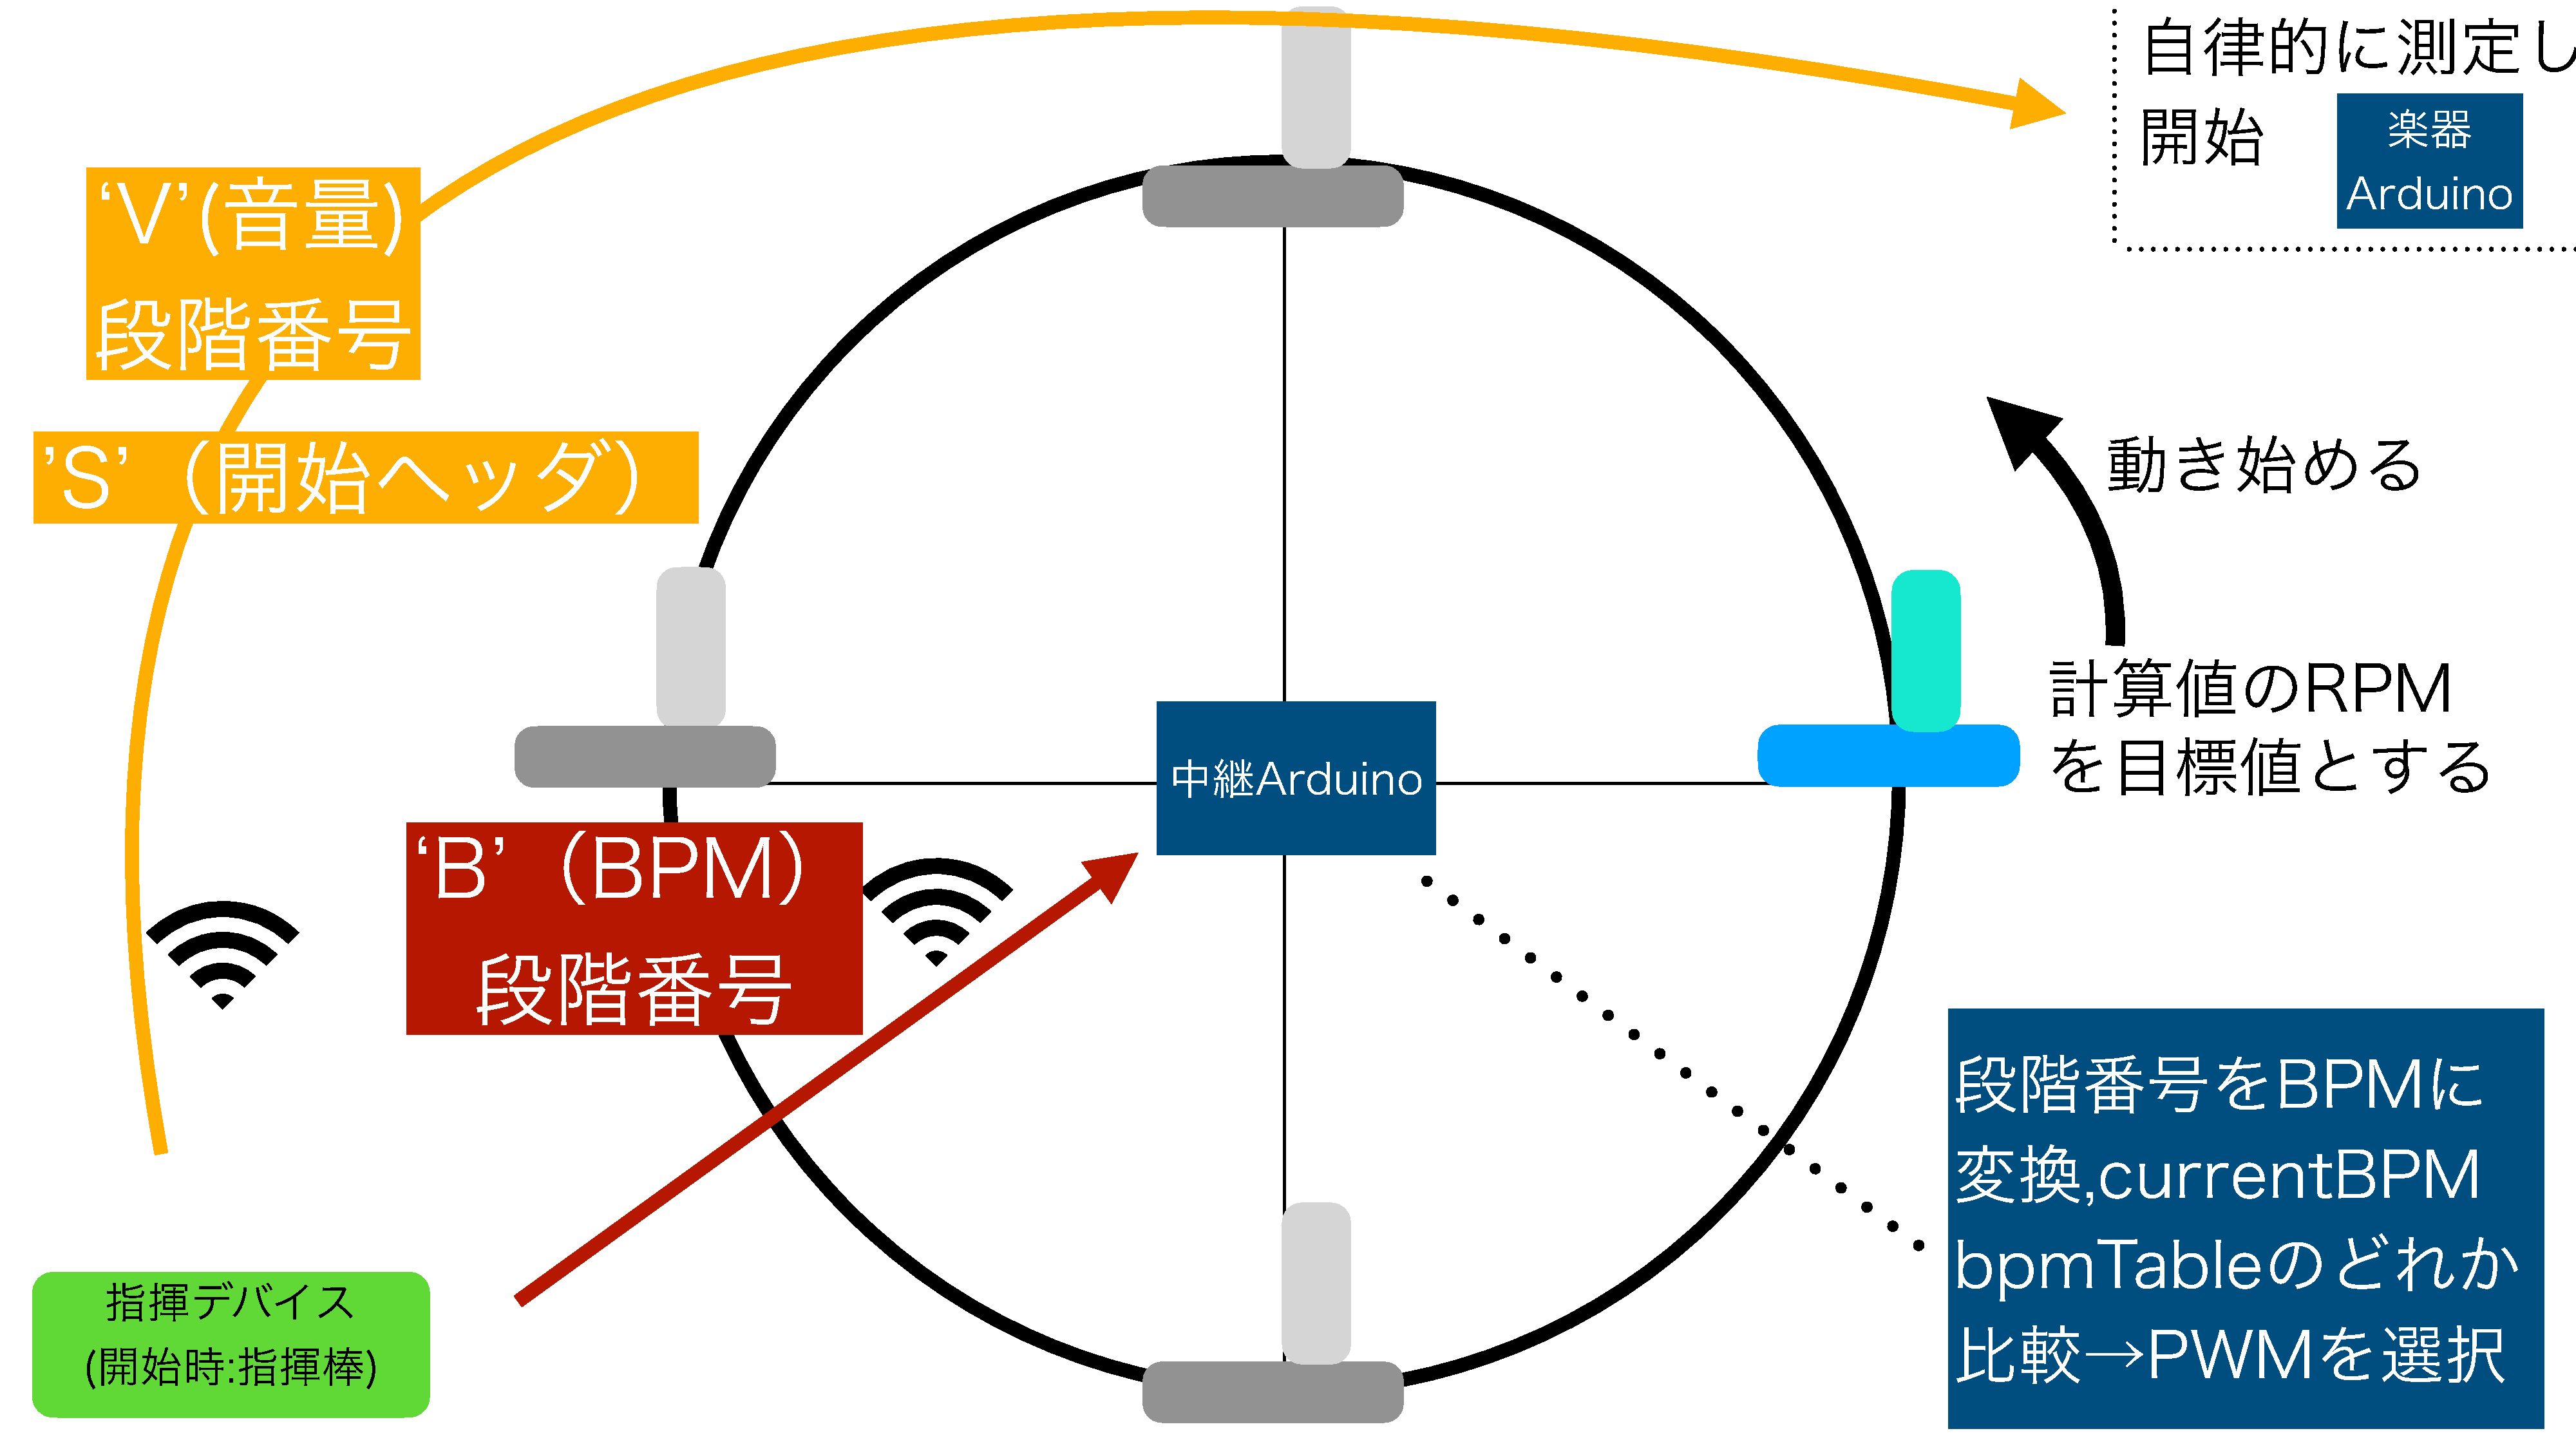
\includegraphics[width=0.8\linewidth]{jusin1.pdf}
  \caption{指揮信号を受信したときの動作と目標RPMへの加速フェーズ．}
  \label{fig:jusin}
\end{figure}
指揮デバイスから受信されたBPMの段階番号は，\texttt{SyncManager::receiveUDP()} を経て，\texttt{MotorControl} クラスへと引き渡される．
\texttt{MotorControl} は，クラス内部の \texttt{bpmTable[]} から該当する実測PWM値を選択し，これをモータの初期速度とする．

観覧車を静止状態から目標速度へ一気に上げると負荷が大きく，リズムの乱れが生じる可能性がある．そのため，本設計では \texttt{MotorControl::startRamp()} を用いて1小節分（4拍分）の時間を加速のための猶予期間として確保する．この猶予の間に\texttt{MotorControl}は目標とする安定した回転速度（RPM）へと到達させるために段階的に加速させる．

観覧車が目標速度に到達したら，その速度で回転を維持する．この期間に，常時点灯している土台のLEDパルスを楽器ユニット側が検知することで，楽器側が自律的にBPMを事前測定するための時間を確保する．
楽器側の測定が完了したときに，指揮デバイス（指揮棒）側の演奏開始操作をトリガーとして合奏を開始する．指揮デバイス側は，カゴが各楽器の正面に届くまでの時間を自身のタイマーから逆算することでモータが安定走行に達した状態と判断できる．そして，各楽器の物理的な配置に合わせて適切な時間差をはさみ演奏開始信号と音量をユニキャストで個別に直接送信する．各楽器ユニットは，このユニキャストによる開始信号を受信した瞬間をトリガーとして一音目を鳴らすことで，正確な発音を開始する設計とする．

\paragraph{BPM（音量）変更設計}
ここでは，演奏中に指揮デバイスから新しいBPM段階番号を受信した場合のロジックを説明する．
本システムでは，実際の回転速度（光パルスの間隔）そのものをBPMの基準としているため，観覧車側は受信した段階番号に応じて即時に回転速度を変更する仕様とする．
具体的には，\texttt{MotorControl} クラスがルックアップテーブルから対応する \texttt{pwmValue} を読み取り，モーターへ反映させる．

本設計では，楽器ユニット側がLEDの物理パルスからリアルタイムにBPMを逆算する構成となっている．そのため，観覧車側の速度が変更された場合でも，楽器側が$n$拍目の光を検知した時刻 $T_n$ とその直前の時刻 $T_{n-1}$ の間隔 $\Delta T = T_n - T_{n-1}$ を用いて，実際の演奏BPM（$BPM_d$）を次式のように算出し，自動的に新しい速度へ追従・同期できる仕様とする．

\begin{equation}
\label{eq:bpmdouki}
BPM_d = \frac{60000}{\Delta T}
\end{equation}


\section{テストの設計}

\subsection{BPM追従テスト}
ここでは，目標とするBPMに対して実際の回転速度がどの程度追従しているかを検証することを目的とする．具体的には，指揮デバイスから各段階のBPMを送信し，観覧車が各目標速度で安定して回転するかを確認する．

\begin{itemize}
    \item 方法: \texttt{MotorControl} クラスがルックアップテーブルから \texttt{pwmValue} を選択し出力する．楽器ユニット側の照度センサがパルスを検知した時間間隔から算出される実測$BPM_d$ が，目標値に対して許容誤差以内であることを確認する．
    \item 合格基準: すべてのBPMにおいて，目標値の $\pm 5\%$ 以内であること．
\end{itemize}

許容誤差の選定にあたっては，聴取者が違和感を抱かない範囲を基準とした．参考文献\cite{ref:tempo1993}によると，単発の音の間隔変化における検知閾値（JND）は平均約 $6\%$ であるが，連続する規則的なシーケンスでは感度が高まり約 $3\%$ となる．また，非音楽家を対象とした実験では，等間隔のシーケンスに対するJNDの平均値は $5.6\%$ と報告されている．したがって，非音楽家を主なターゲット層と想定する場合，$\pm 5\%$ 程度がほとんどの人が変化に気づかない妥当な合格基準であると考え，設定した．

\subsection{同期精度テスト}
ここでは，物理的な動きと楽器の発音タイミングがどの程度一致しているかを検証することを目的とする．具体的には，観覧車のLEDが照度センサを通過する物理的なタイミングと，楽器側の発音タイミングが一致し，許容範囲内の遅延におさまっているかを確認する．

\begin{itemize}
    \item 方法: LEDの通過時刻と，楽器ユニットが音声を出力したタイミングの差分をオシロスコープ等で測定する．
    \item 合格基準: LED検知から発音までの遅延が 50 ms 以内であること．
\end{itemize}

各楽器の発音が一体として知覚されるためには，同期のズレを許容範囲内に抑える必要がある．先行研究\cite{ref:haas1951}では，意図しない離散的反射音（エコー）として認識される遅延は 50 ms を超える場合に発生することが示されている．この知見に基づき，本システムでは通信・処理の合計遅延時間を 50 ms 以内に収めることを設計目標とした．

\subsection{負荷テスト}
ここでは，システムに高負荷をかけた際の挙動の安定性を検証する．

\begin{itemize}
    \item 検証1（通信負荷）: BPMや音量の変更パケットを短時間で連続してユニキャストし，\texttt{SyncManager::receiveUDP()} における通信の取りこぼしやフリーズが発生しないかを確認する．
    \item 検証2（物理負荷）: 最大速度（180 BPM）で長時間連続運転を行い，モータなどの過熱による影響を確認する．
    \item 合格基準: 高負荷状態においても，システムが停止したり制御不能に陥ったりしないこと．
\end{itemize}

\newpage
\begin{thebibliography}{999}

\bibitem{ref:Arduino_wifi} Arduino WiFi Library, wl\_definitions.h,, \url{https://github.com/arduino-libraries/WiFi/blob/master/src/utility/wl_definitions.h}, (参照 2026-05-08).

\bibitem{ref:Arduino_memori} Arduino, "Arduino UNO R4 WiFi Datasheet", \url{https://docs.arduino.cc/resources/datasheets/ABX00087-datasheet.pdf}, (参照 2026-04-28).

\bibitem{ref:control}
Control.com, ``DC Motor Speed Control,'' {\em Lessons In Electric Circuits}, \\
\url{https://control.com/textbook/variable-speed-motor-controls/dc-motor-speed-control/}，（参照 2026-05-04）．

\bibitem{ref:tempo1993}
C.~Drake and M.~C.~Botte,
``Tempo sensitivity in auditory sequences: Evidence for a multiple-look model,''
\textit{Perception \& Psychophysics},
vol.~54,
no.~3,
pp.~277--286,
1993.

\bibitem{ref:haas1951}
H.~Haas,
``\"Uber den Einfluss eines Einfachechos auf die H\"orsamkeit von Sprache,''
\textit{Acustica},
vol.~1,
pp.~49--58,
1951.

\end{thebibliography}
\end{document}